\documentclass{article}
\usepackage{CJKutf8, indentfirst, graphicx, subfigure}
\begin{document}
\begin{CJK}{UTF8}{bsmi}
\title{硬體設計與實驗 Lab5 Report}
\author{104021219 鄭余玄}
\date{}
\maketitle
\section{實做過程}
lab5 就如同之前的 lab,
會需要重複使用之前的 module,
像是 clock\_divider, debounce circuit
和七段顯示器。
而 onepulse 電路基本上是照老師投影片的作法。
lab5.xdc 也只需要依照規定接一接就行了。

lab5 一開始需要先把訊號 debounce 之後,
再接到 onepulse 電路,這樣壓下一次按鈕,
才能夠正確地判斷為一次的按壓。
FSM 的狀態我是依照助教提供的方法分成四種,
前後兩種 clk 分別是除以 $2^{16}$ 和 $2^{25}$,
再使用組合電路來選擇 FSM 現在的 clock。

組合電路判斷 next state 的程式碼中,
先把 next state 設成當前狀態(state),
再用 case 判斷當前狀態(state),
如果已經達到可以改變狀態,
則更改 next state。
而且優先序高的動作放在 if 越前面的判斷,
像是 cancel 就會先比投錢優先判斷。
按照這的原則,就能很有條理的完成了。
此外,投錢的方法我是逐位判斷,
買票扣錢也是。
\subsection{FSM diagram}
\begin{figure*}[h]
\centering{
\hfill
  \subfigure[]{ \label{fig:fsm}
    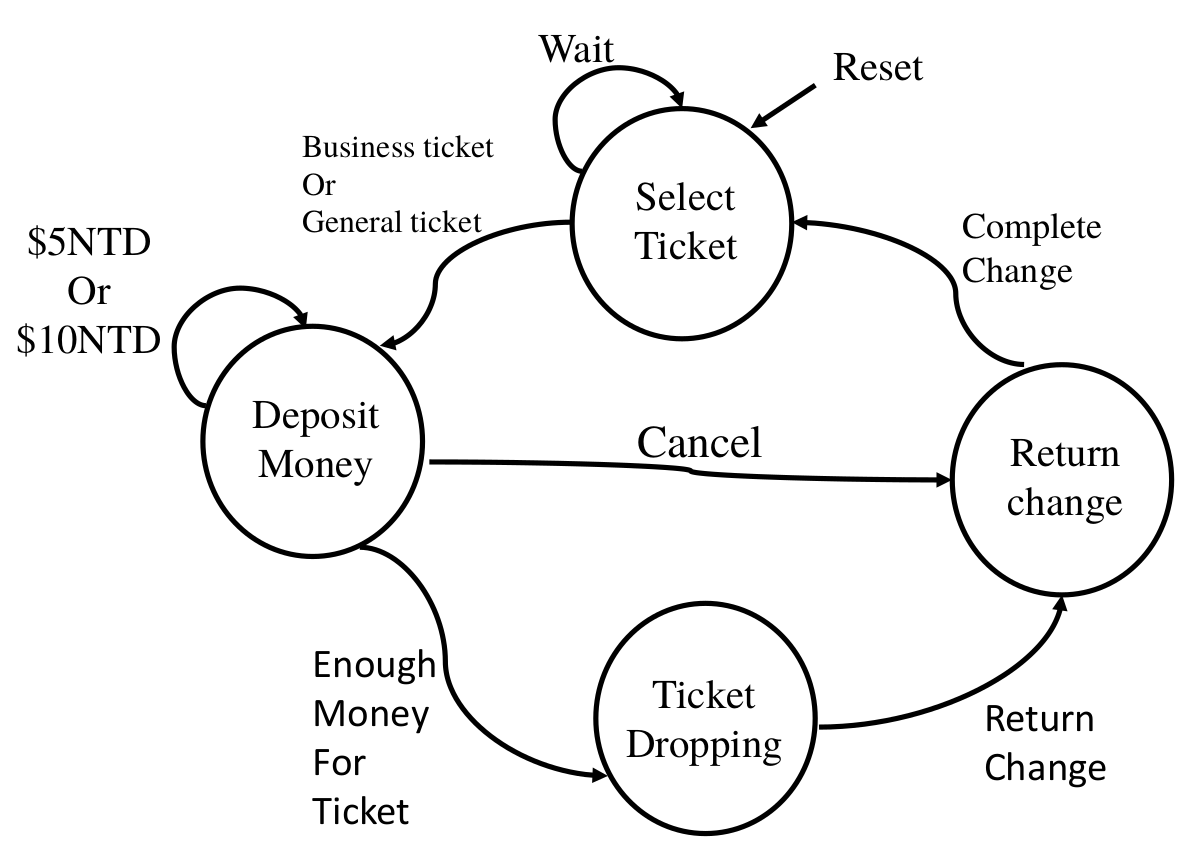
\includegraphics[width=.8\textwidth, angle=0]{lab5}
  }
}
\caption{lab5 Finite-State Machine}
\end{figure*}
雖然這次助教沒有提供 block diagram,
但是 FSM 的狀態圖也有很大的幫助。

\section{學到的東西及遇到的困難}
這次學到的就是 onepulse 電路這個概念,
前一個 lab 因為只有 enable 訊號控制,
所以不會在跑 FSM 的時候又壓按鍵控制,
因此不需要產生 onepulse。
而在這次 lab 中就非常重要,
因為要讓 clock 能夠讀到,
卻不能多讀或是讀不到,
所以就需要在加上 onepulse 電路。

這次遇到的困難就是投影片好像沒有說清楚,
前兩個狀態和後兩個狀態的 clock 頻率不同,
導致我在寫的時候發覺 onepulse 似乎沒有用,
也在 demo 前和助教研究了很久
(謝謝助教!!),
最後才發現原來是 clock 弄錯了。

\section{想對老師或助教說的話}
我覺得 lab 少了 block diagram 難度就增加了,
因為在寫錯的時候,
就會開始懷疑自己有沒有接錯線,
像是之前助教有提供,
就會比較專注在邏輯的問題上。

\end{CJK}
\end{document}
